\section{Video platforms}
\label{sec:Video platforms}

The initial phase of the thesis project has been dedicated to the research of the different platforms of streaming video in order to highlight the strengths, differences and cost required. As already alluded in the next section briefly describes the features, services and costs of major video platforms, even though the final choice was to focus the argument on the development of a video platform independent through the use of services offered by Amazon AWS.


\subsection{Video classification }
\label{sec:Video classification}

\begin{itemize}
\item JW Player is an open source solution, allowing anyone with a website to replace the simple embedded from youtube with a real player:

\begin{itemize}
\item Customizable
\item Reliable
\item Scalable
\item Compatible with different CMS via plugin
\item Free or Paid
\item Complete set API
JW Player supports playback of any format the Adobe Flash Player and HTML5 and reads compressed formats such as (FLV, H.264, MP4, VP8, WebM, MP3, AAC, JPG, PNG and GIF), besides supports content such as video streaming and live webcasting (RTMP, HTTP) and all CDN and switcher adaptive bitrate allows the distribution and playback of high-quality content.
\end{itemize}


\begin{figure}[htb]
 \centering
 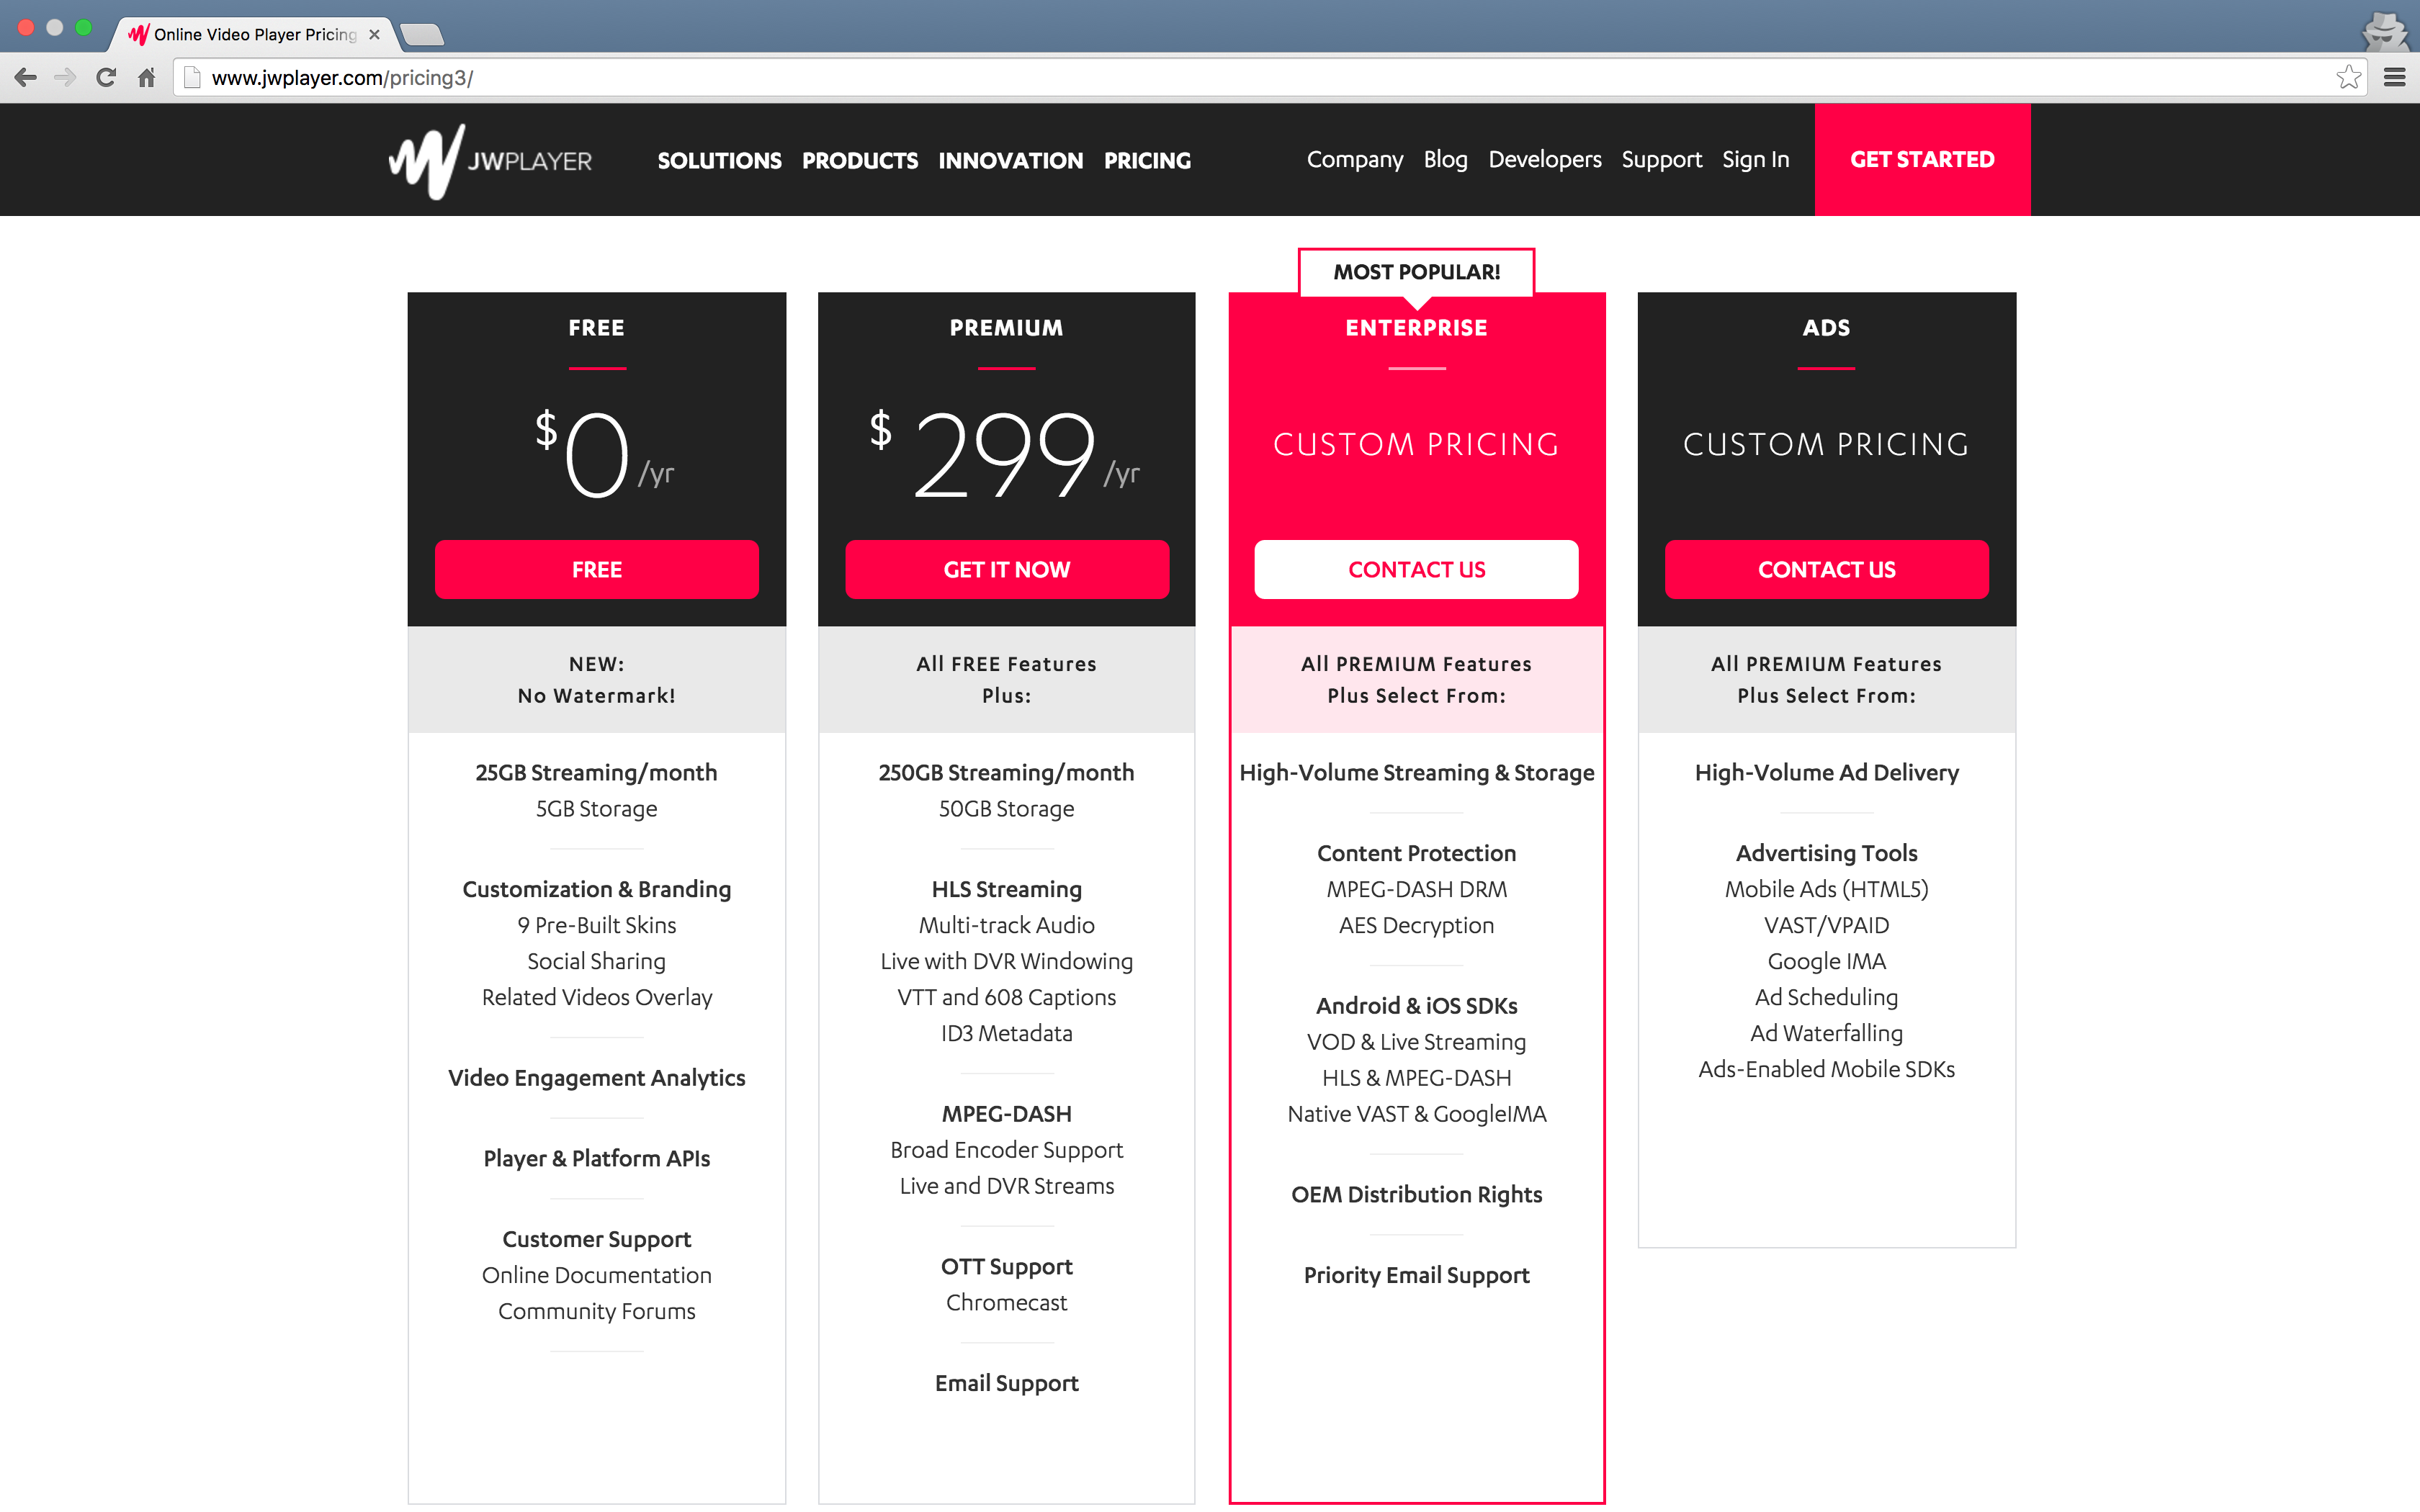
\includegraphics[width=1.0\linewidth]{images/chapter3/jwtPLayer.png}\hfill
 \caption[JW player cost]{JW player cost}
 \label{fig:fourV}
\end{figure}

\newpage 

\item The server Video Wowza is based on the platform streaming web TV Wowza Streaming Engine and is supplied with a control panel complete with:
\begin{itemize}

\item server settings Wowza
\item Quick links for different readers of Streaming
\item Player HTML5 to be included in the pages of your site (it works on fixed and mobile platforms)
\item Traffic statistics historical server
\item Statistics in real time of connected users with geolocation. The service is configurable in different bit rate depending on the needs of video quality:
\item 256 kbs - For a low resolution quality but accessible from mobile devices
\item 512 kbs - For a HQ quality standards equivalent to a normal television flow
\item 720 kbs - For HD quality videos
\item 1048 kbs - For a quality FULL HD video
\end{itemize}

You can send the video stream using any encoder that supports Wowza streaming server.


\begin{figure}[!htb]
 \centering
 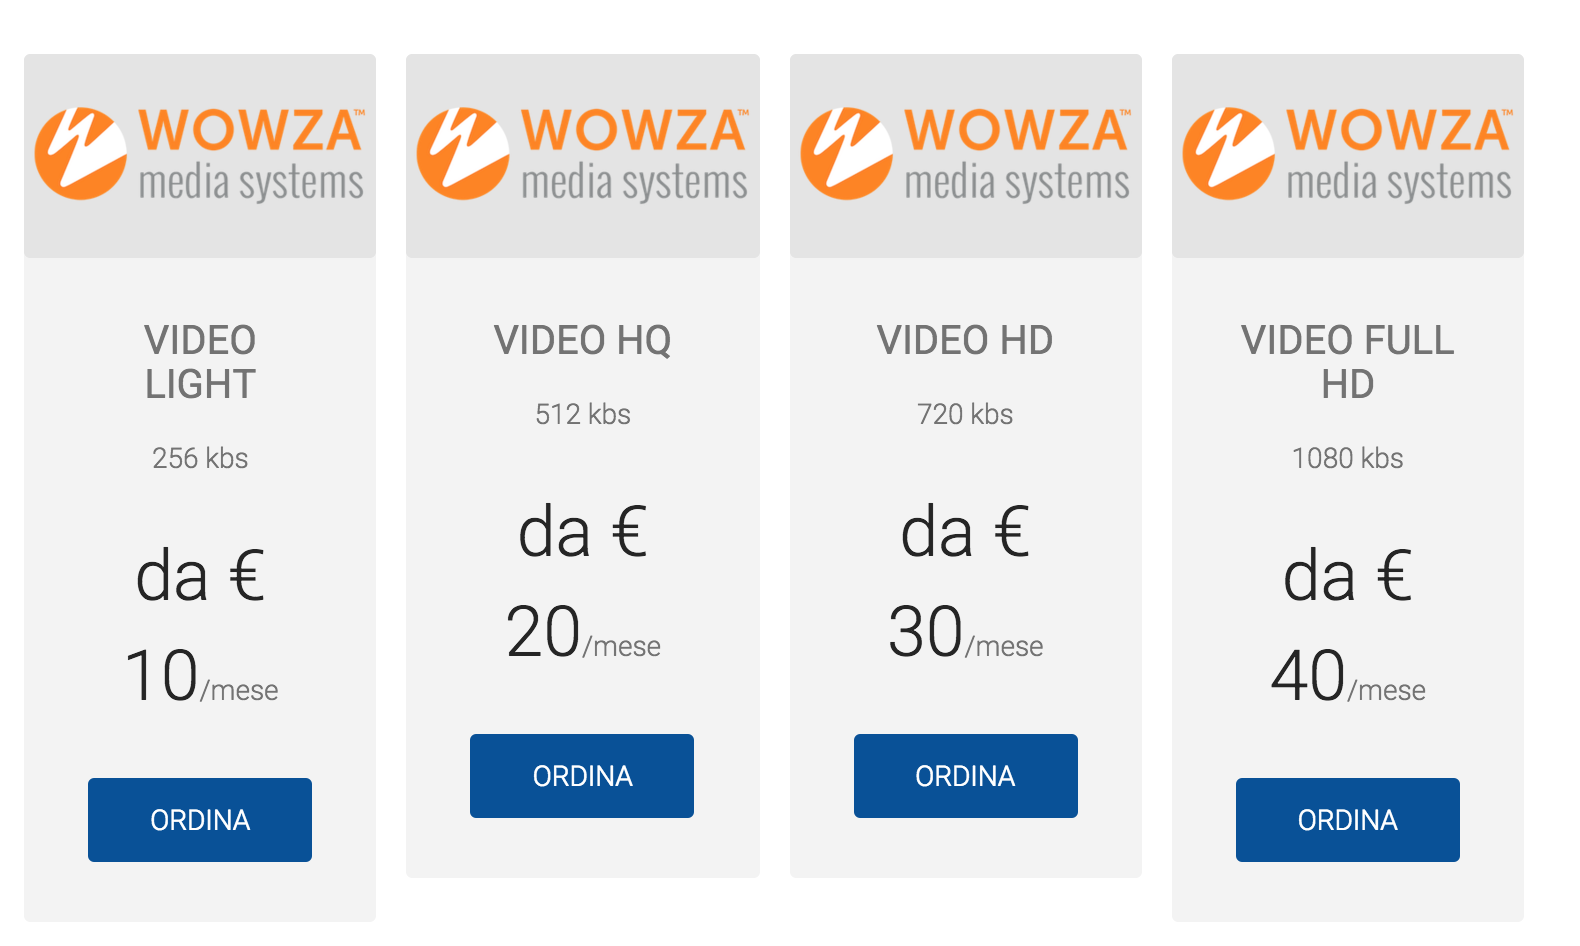
\includegraphics[width=1.0\linewidth]{images/chapter3/wowza.png}\hfill
 \caption[Wowza cost]{Wowza cost}
 \label{fig:fourV}
\end{figure}

\item Ustream is a broadcast platform for live streaming of events of any kind: from news conferences to product launches, from classes via teleconference to international protests.

Users can create through their computer and a standard Web browser or a smartphone, via app for iOS and Android systems, broadcast channel.
Users also can register their events and then load them on the platform, so that they can be broadcast at a later date. With the use of special cameras also Ustream makes it possible to stream HD video.
During the direct viewers can interact with each other through chat and answer surveys and questionnaires posed by the organizers of the stream.

\end{itemize}
  
 \begin{figure}[!htb]
 \centering
 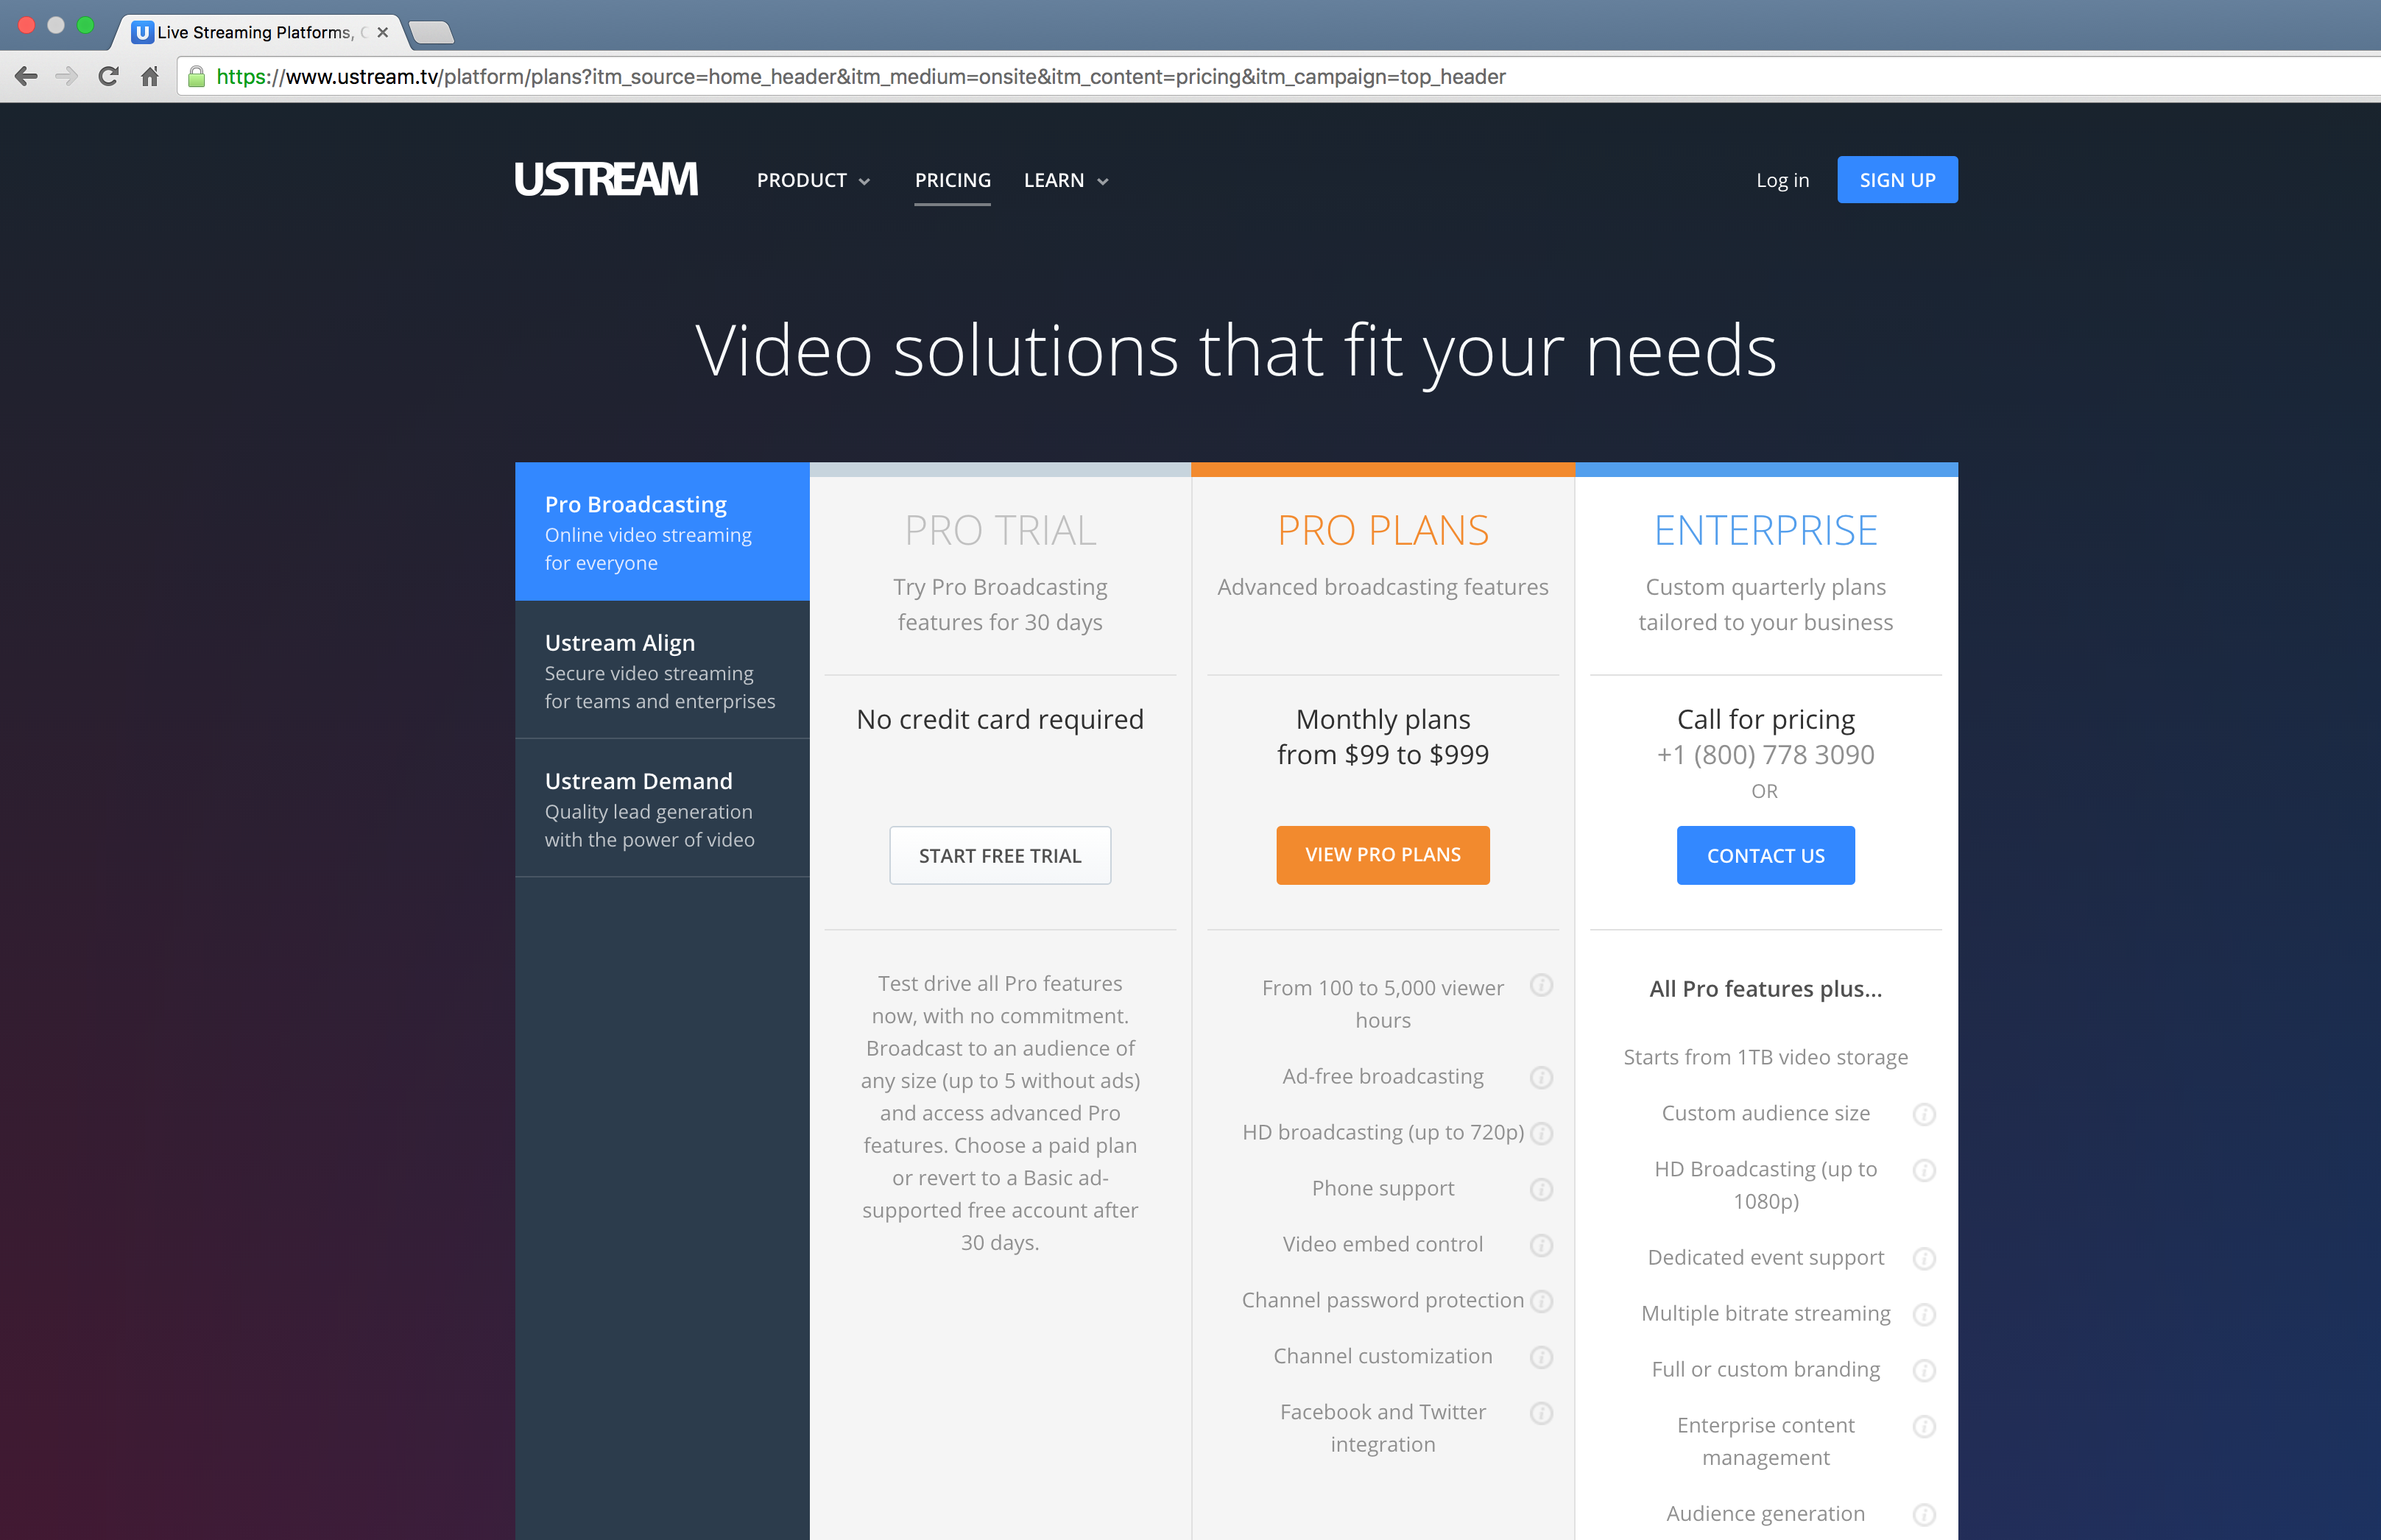
\includegraphics[width=1.0\linewidth]{images/chapter3/ustream.png}\hfill
 \caption[Ustream cost]{Ustream cost}
 \label{fig:fourV}
\end{figure}